\chapter{The Debugging Challenge} \label{chap3}

\section{Introduction}

In this chapter we first provide an overview of the record-and-replay
approach for debugging a class of non-deterministic applications and
describe the properties of existing record-and-replay tools. We then
present our extension to the record-and-replay approach together with
the performance of the integration of our extension into a
production-grade record-and-replay tool.

\section{Record-and-Replay Approach and Tools} 

To overcome the impediments to debugging associated with
non-deterministic executions, a class of debugging aids collectively
referred to as record-and-replay tools have been developed. These
tools allow developers to record one execution of a target
application, then replay it exactly. In general, record-and-replay
tools must establish an order of events during the recorded execution,
then write a representation of that order to some form of persistent
storage. The exact data that must be recorded depend on what
assumptions can be made about the form of nondeterminism the target
application exhibits. Figure~\ref{fig:rrframework} shows a general
overview of these tools' framework.
\begin{figure}[!ht]
    \centering
    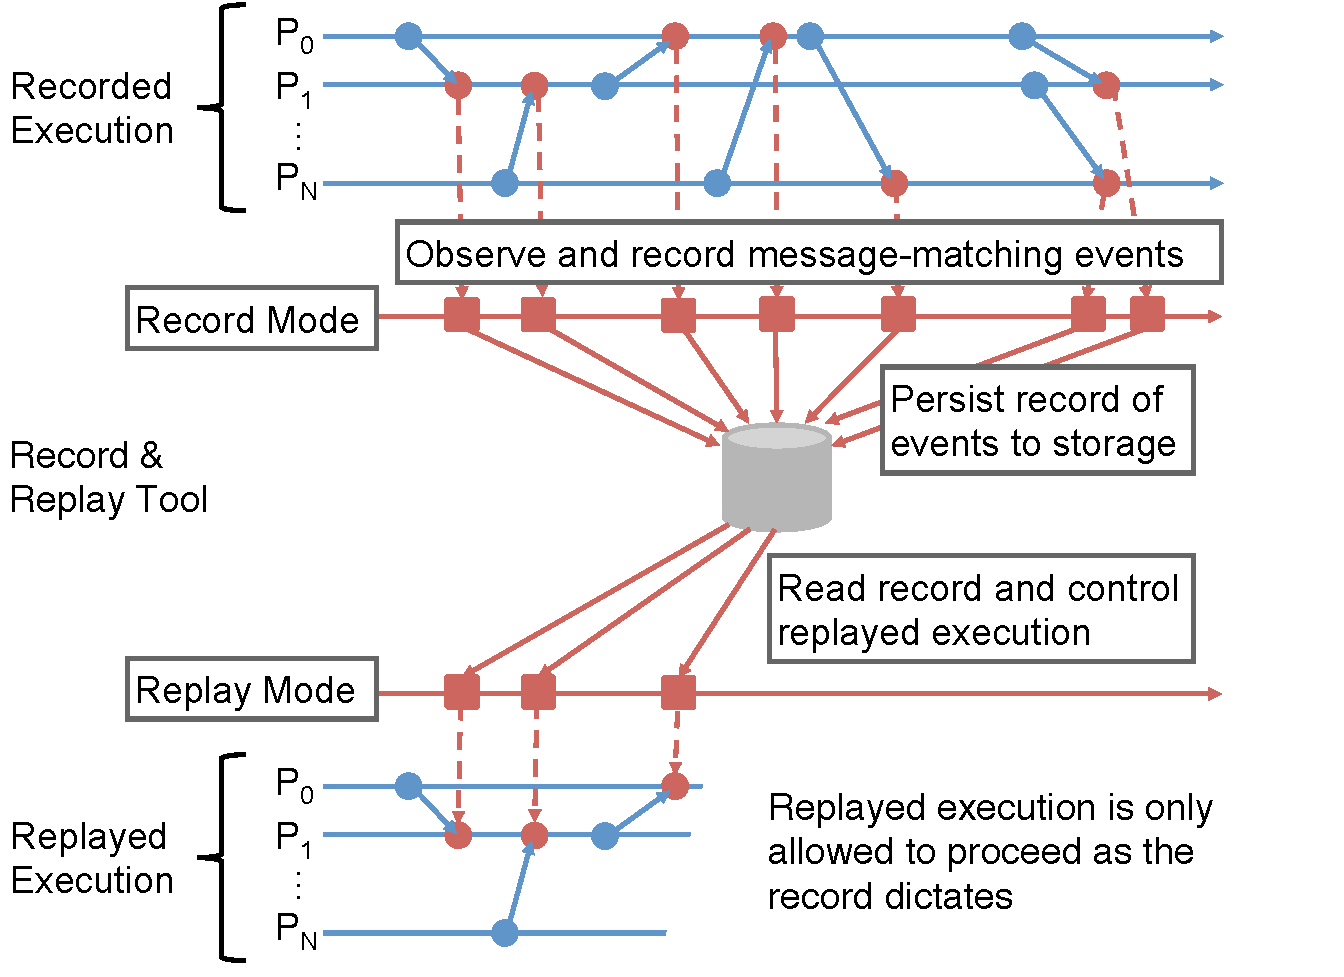
\includegraphics[width=0.8\linewidth]{chapter_3_figures/rrframework.pdf}
    \caption{General overview of a record-and-replay framework.}
    \label{fig:rrframework}
\end{figure}

Necessary behaviors of record-and-replay tools can be sorted in two
groups: during recording and during replay. During recording, a tool
must observe communication events in an application's execution and
store (or write) information that unambiguously orders the observed
events into a record. One way to do this task is with logical clocks
and metadata (described in the next section). Metadata in message
passing applications include processes' rank, tag, and communication
event type (e.g., completion of a receive vs. invocation of
Test-family function).

During replay, a tool must read (or query) the record followed by
buffering and re-ordering communication events in the subsequent
execution. Correctness of the replay depends on assumptions about the 
application (e.g., is the application send-deterministic)~\cite{CommunicationDeterminism:Cappello:2010}
and inductive arguments (e.g., the $n^{th}$ event is replayed correctly as a
consequence of the $n-1^{th}$ event being replayed correctly).

Existing record-and-replay tools fall into two broad categories:
data-replay and order-replay. These categories refer to the content
that is traced by the tool during recording.  Specifically,
data-replay tools record the total content of messages, whereas
order-replay tools opt instead to record the messages' relative
ordering. The state of the art in record-and-replay takes the
order-replay approach primarily due to the significant reduction in
record size it provides by not recording possibly large message
payloads in addition to the necessary message order data.

The earliest record-and-replay tools employed the data-replay
approach, but attempt to mitigate the growth of record size via
selectively recording only those messages deemed at runtime to be a
source of non-determinism.  Netzer and Miller employ vector clocks to
identify racing messages and thus restrict the number of necessarily
recorded messages in their tool~\cite{OptimalTracing:Netzer:1992}.
Later work by Cl\'emec\c on \textit{et al.} used a similar vector
clock approach, but extended the tool's capabilities to record
non-blocking probes as well as wildcard
receives~\cite{RaceDetection:Clemencon:1995}. Despite these
techniques' applicability at the time of their creation, their use of
vector clocks makes them prohibitively expensive for modern HPC
systems, since each message is saddled with a vector of $n$ elements
where $n$ is the number of processors in the
system~\cite{VectorClocksI:Fidge:1988}.

Later record-and-replay tools embraced the order-replay design,
recognizing that despite the need to make stronger assumptions about
message contents than data replay tools do, increasingly large systems
necessitate the smaller record sizes that order-replay tools can
deliver.  One early tool in this domain was the Nondeterministic
Program Evaluator (NOPE) developed by Kranzlm\"uller and
Volkert~\cite{NOPE:Kranzlmuller:1999}. Last, Clock-Delta Compression
(CDC)~\cite{ClockDeltaCompression:Sato:2015} is the state-of-the-art
approach to record-and-replay that aims to overcome the problem of
large record size that renders traditional record-and-replay
techniques inapplicable at extreme scale. We build our work on top of
this approach that we describe in the next section.

\section{Clock-Delta Compression}

Clock-Delta Compression (CDC) establishes an order on communication
events during recording by piggybacking logical clocks on messages
between processes, and applies a novel compression pipeline to the
record that leverages properties of the piggybacked clocks. In this
section, we provide an overview of the CDC record format, a high-level
description of the compression pipeline, and describe the role of the
piggybacked logical clocks with respect to the record format and the
compression pipeline.

The CDC record format is a data structure built up during recording
that contains sufficient information about interprocess communication
events to enable deterministic replay of the recorded execution. The
record format consists of three main parts: the
\textit{with-next-table}, the \textit{unmatched-test-table} and the
\textit{matched-test-table}. The \textit{with-next-table} records when
multiple incoming messages match with a single receive request, as can
occur if MPI\_Testsome, MPI\_Testall, MPI\_Waitsome, or MPI\_Waitall
are employed by the application.  The \textit{unmatched-test-table}
records instances of MPI\_Test-family functions being called on a
receive request when no matching send exists, as can occur when a
polling loop of test calls is used to complete a non-blocking
receive. Finally, the \textit{matched-test-table} records the actual
matches between receive requests and incoming messages. This component
of the record format is our focus since the most dramatic reductions
in record size that CDC offers apply to the
\textit{matched-test-table}. Moreover, the specific implementation of
the underlying logical clock protocol directly effects the
compressibility of the \textit{matched-test-table}.

The CDC compression pipeline is applied to the CDC record format
during recording and consists of three stages: permutation encoding,
linear-predictive encoding (LPE), and lossless compression. The
permutation encoding stage is applied only to the
\textit{matched-test-table}, whereas LPE is applied to components of
the \textit{matched-test-table} and \textit{unmatched-test-table}. The
lossless compression stage is applied to the entire record after
permutation encoding and LPE. We provide the description of the
algorithm for permutation encoding in
Section~\ref{sec:permutation_encoding} due to the critical reduction
in size of the \textit{matched-test-table} that it provides and the
degree to which its functionality is intertwined with the notion of a
logical clock ticking policy described in Section
~\ref{sec:logical_clocks}.

\section{Logical Clocks} \label{sec:logical_clocks}

Logical clocks, originally defined by Lamport
in~\cite{LogicalClocks:Lamport:1978}, provide a method for
establishing a partial order on events in a distributed system. Within
the context of the CDC record-and-replay technique, we describe 
the rules of the logical clock protocol that CDC employs, we define
the notion of logical clock ticking policy, and we discuss how
recording events are distinguished by the logical clock values
associated to them.

CDC establishes a partial order on all communication events that occur
during recording by maintaining in each process $p$ an integer value
referred to as the local clock of that process.  Whenever $p$ sends a
message to another process, $p$ attaches a copy of its local clock to
the message, then increments its local clock by some value $t$,
hereafter referred to as a ``tick''.  When another process $q$ receives
$p$'s message, it sets its own local clock to the maximum of its
current value and the value attached to the message it just
received. Then $q$ increments its local clock by some amount (i.e.,
$q$ ticks its local clock). Two immediate consequences of this
protocol are that within a process, if an event $e_0$ occurred before
another event $e_1$, the logical clock values associated to those
events (e.g., $c_0$ and $c_1$) satisfy $c_0 < c_1$, and between a
sender process and a receiver process, a send event's clock will
always be less than its corresponding receive event's clock.

So far we have discussed logical clocks' ticks without specifying what
values they must take. In Lamport's paper on logical
clocks~\cite{LogicalClocks:Lamport:1978}, ticks are assumed to always
equal $1$, but in fact all that is necessary to establish a partial
order is that the ticks have positive value. In the context of
record-and-replay, since the replayed execution must exactly match the
recorded execution, we require the additional constraint that the
ticks be deterministic (i.e., during replay), for all processes, the
$i$th tick applied to a process's local clock must match the $i$th
tick that was applied to its local clock during recording. We define a
\textit{logical clock ticking policy} to be a mechanism for deciding
what value each tick applied to each process's logical clock will
take.

\section{In- and Out-of-order Received Messages}

In this section, we define the concept of an event (e.g., message
receive) being in-order or out-of-order with respect a logical clock
reference order, and how out-of-order messages impact the size of the
\textit{matched-test-table}. In CDC, every receive completion event is
associated to a logical clock value that is piggybacked on a received
message. Specifically, each process has a ``local clock'' (LC) that is
initially zero. When a process (e.g., $P_0$) sends a message, its LC
is attached to the message as the ``sent clock'' (SC). Afterward, the
sending process's LC is incremented by one. When a process (e.g.,
$P_1$) receives a message from another process (e.g., $P_0$), it
updates its LC by the Lamport Clock protocol $LC = max(LC, SC) + 1$
and records the receive event. The list of SC values that every
receiving process builds up over the course of recording an execution
defines whether a received message is in-order or out-of order: if the
new SC is larger than the previous received SC, then the message is
in-order; if it is smaller, then then the message is
out-of-order. The SC values are the input to the permutation
encoding step of the CDC compression pipeline, and the degree of
monotonicity in this list of values determines the effectiveness of
the compression. Moreover, the list of SC values is not the same
logical clock value that any receiving process updates its local clock
to, and as such does not impose a partial order on events in the same
way. Figure~\ref{fig:inandout} shows examples of in-order or
out-of-order messages: Figure~\ref{fig:inandout}.(a) shows an example
of an in-order received message and Figure~\ref{fig:inandout}.(b) shows
an example of an out-of-order received message. In
Figure~\ref{fig:inandout}.(a), the SC of $P_0$ is 17; because the SC
value is larger than the precious SC of $P_1$ (in the figure the
$SC_{previous}$ is 15), the received in-order message is annotated in
the SC list but will not be recorded in the \textit{matched-test
  table}. This is not the case in Figure~\ref{fig:inandout}.(b) in
which the the SC of the sending $P_0$ is still 17 but the previously
annotated SC is larger (i.e., equal to 19), causing the recording of
the event in the \textit{matched-test table}.
\begin{figure}[!htb]
\centering
\minipage[t]{0.45\textwidth}
\begin{tabular}{c}
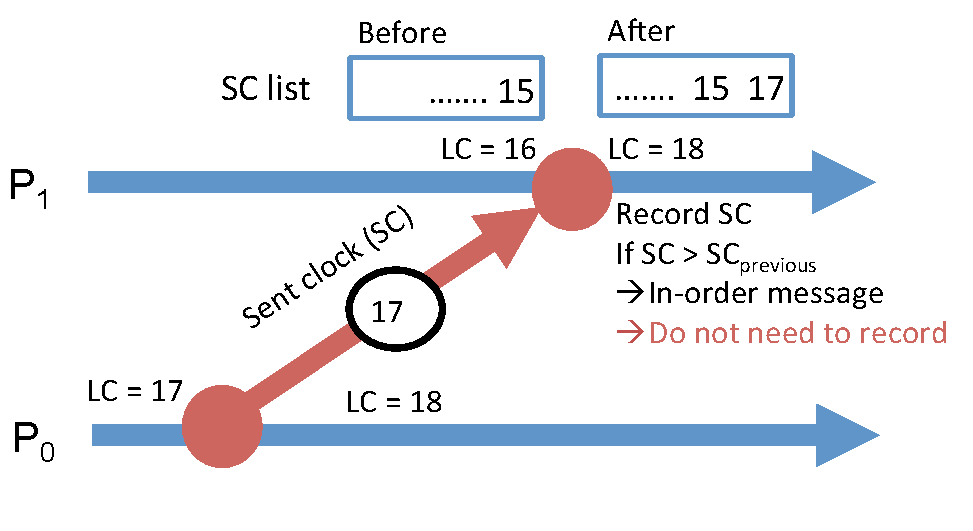
\includegraphics[width=\textwidth,
  height=6cm]{chapter_3_figures/inorder.pdf} \\ (a) In-order \\
\end{tabular}
\endminipage
\minipage[t]{0.45\textwidth}
\begin{tabular}{c}
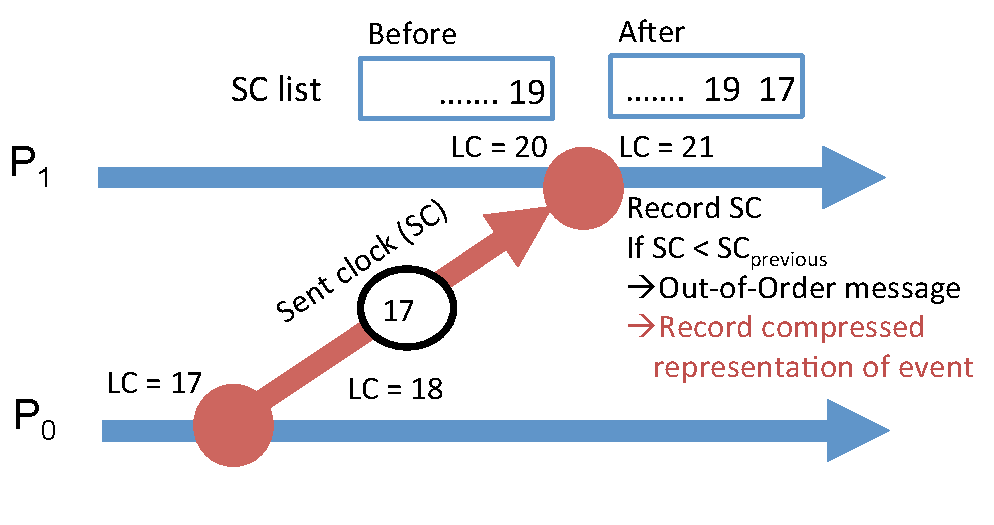
\includegraphics[width=\textwidth,
  height=6cm]{chapter_3_figures/outoforder.pdf} \\ (b) Out-of-order\\
\end{tabular}
\endminipage
\caption{Example of in-order (a) and out-of-order (b) messages.}
\label{fig:inandout}
\end{figure}

Figure~\ref{fig:exampleinandout} show a larger five-stage example in
which multiple messages are received by a process $P_0$. For each
stage, the upper figure shows the snapshot with the sent and received
messages up to that point for process $P_0$; the bottom figure shows
the associated SC list. In Stage 1, $P_0$ receives a message from, for
example, $P_1$. $P_0$ updates its local clock (LC), which was
initially equal to 1, by using the Lamport Clock protocol to 4 (i.e.,
LC of $P_0$ becomes the max of LC and SC plus one) and temporally
records the time of the received message (i.e., SC time is equal to
3). In Stage 2, $P_0$ receives a second message from $P_2$; $P_0$
updates its LC following the same procedure as in Stage 1. The LC of
$P_0$ becomes 6 and the process also records the received SC value (in
this case SC is equal to 5). We observe that at the end of Stage 2 the
received clocks' values are monotonically increasing ``in-order''. The
process takes note of the message's SC but does not forward the SC
value to its \textit{matched-test table}. In Stage 3, $P_0$ sends
messages. Its LC increases each time a send is initiated but no
clock is recorded. In Stage 5, two additional messages from a
different process than $P_1$ are received by $P_0$. This time the
first message is out-of-order (i.e., with a SC equal to 4 smaller than
5) and is thus used for building the process'~\textit{matched-test
  table}. The second is in-order (i.e., with a SC equal to 7 larger
than 4) and is not considered for the process'~\textit{matched-test
  table}.
\begin{figure} [!htb]
    \centering
    \begin{minipage}{0.20\textwidth}
        \includegraphics[width=0.9\linewidth]{chapter_3_figures/record_step_2}
        \label{fig:record_step_2}
    \end{minipage}%
    \begin{minipage}{0.20\textwidth}
        \includegraphics[width=0.9\linewidth]{chapter_3_figures/record_step_3}
        \label{fig:record_step_3}
    \end{minipage}% 
   \begin{minipage}{0.20\textwidth}
        \includegraphics[width=0.9\linewidth]{chapter_3_figures/record_step_4}
        \label{fig:record_step_4}
    \end{minipage}%
    \begin{minipage}{0.20\textwidth}
        \includegraphics[width=0.9\linewidth]{chapter_3_figures/record_step_5}
        \label{fig:record_step_5}
    \end{minipage}%
    \begin{minipage}{0.20\textwidth}
        \includegraphics[width=0.9\linewidth]{chapter_3_figures/record_step_6}
        \label{fig:record_step_6}
    \end{minipage}%
\\
    \begin{minipage}{0.20\textwidth}
        \stackunder[5pt]{\includegraphics[width=\linewidth]{chapter_3_figures/received_clocks_2}}{Stage 1}
        \label{fig:received_clocks_2}
    \end{minipage}%
    \begin{minipage}{0.20\textwidth}
        \stackunder[5pt]{\includegraphics[width=\linewidth]{chapter_3_figures/received_clocks_3}}{Stage 2}
        \label{fig:received_clocks_3}
    \end{minipage}%
    \begin{minipage}{0.20\textwidth}
        \stackunder[5pt]{\includegraphics[width=\linewidth]{chapter_3_figures/received_clocks_4}}{Stage 3}
        \label{fig:received_clocks_4}
    \end{minipage}%
    \begin{minipage}{0.20\textwidth}
        \stackunder[5pt]{\includegraphics[width=\linewidth]{chapter_3_figures/received_clocks_5}}{Stage 4}
        \label{fig:received_clocks_5}
    \end{minipage}%
    \begin{minipage}{0.20\textwidth}
        \stackunder[5pt]{\includegraphics[width=\linewidth]{chapter_3_figures/received_clocks_6}}{Stage 5}
        \label{fig:received_clocks_6}
    \end{minipage}%
    \caption{Example of a five-stage execution in which in-order and out-of-order
      messages are received by process $P_0$. We show in-order receives in stages 
      1, 2, 3, and 5. We show an out-of-order receive in stage 4, in which a sent
      clock of 4 is received after $P_0$ has already received a larger sent clock
      of 5.}
    \label{fig:exampleinandout}
\end{figure}

\section{Permutation Encoding} 
\label{sec:permutation_encoding}

During recording, the process receiving messages with the attached
logical clock values builds up the \textit{matched-test table}. The
table collects only information on out-of-order messages and
therefore, the number of out-of-order messages determines the size of
the \textit{matched-test table}.

Sato \textit{et al.}  made the observation that for most processes,
the list of received clock values tended to consist of values that
were nearly-sorted in increasing order (i.e., in-order messages), as
show in the authors'
manuscript~\cite{ClockDeltaCompression:Sato:2015}.  The observed
similarity between the actual order of received clock values (referred
to hereafter as the observed order) and the ordering of received clock
values in ascending order (referred to hereafter as the logical clock
reference order) suggests that there is a compact way of representing
the difference between the observed order and the reference
order. This difference, which can be thought of as the permutation
that maps the reference order to the observed order, is what the
permutation encoding stage computes.  Representing the
\textit{matched-test table} by this permutation suffices for replay
because during replay, messages arriving in arbitrary order can be
buffered, sorted based on their piggybacked logical clock values into
the reference order, and then \textit{un-sorted} into exactly the
observed order from recording by applying the recorded permutation.

The permutation encoding stage works by computing a minimal set of
edits that effectively map the logical clock reference order back to
the observed order. Each edit is represented as a pair of integers
(i.e., an index and an offset). Consider that if a process receives
all its inbound messages such that their piggybacked logical clock
values are received in strictly ascending order, then the observed
order and the logical clock reference order are identical (i.e., all
messages are received in-order). Since permutation encoding is an
effective compression technique to the extent that the observed order
is similar to the logical clock reference order, a reduction in the
number of out-of-order message receives translates to a reduction in
the size of the \textit{matched-test table}, and consequently a
reduction in the size of the total record.
Figure~\ref{fig:encoding_example} shows how, for the example in
Figure~\ref{fig:exampleinandout}, we need to swap only the 2nd and 3rd
message receives to create our observed sequence of messages starting
from a totally in-order set of message. Therefore, ``swap(2,3)'' is
written to the \textit{matched-test table} for $P_0$ and everything
else is discarded.
\begin{figure}[!htb]
    \centering
    \includegraphics[width=0.9\linewidth]{chapter_3_figures/encoding_example}
    \caption{Process to transform a totally in-order set of message
      receives into the order we observed for
      Figure~\ref{fig:exampleinandout}.}
    \label{fig:encoding_example}
\end{figure}

During the replay stage, a record-and-replay tool buffers incoming
messages and re-orders them so that the processes receive the messages
in the same order the processes did during the recorded
execution. Figure~\ref{fig:replay_example} shows the the steps
followed by the replay stage for the example in
Figure~\ref{fig:exampleinandout}.
\begin{figure}[!htb]
    \centering
    \includegraphics[width=0.9\linewidth]{chapter_3_figures/replayexample.pdf}
    \caption{Steps performed by the replay stage in a record-and-replay
      tool to recreate the observed execution built during the record
      stage.}
    \label{fig:replay_example}
\end{figure}

\section{Logical Clock Ticking Policies}

To minimize the size of the matched-test table, and hence the size of
the overall record, it is necessary to minimize the number of messages
that are received out-of-order. Sato \textit{et al.} propose to
accomplish this minimization by means of a logical clock ticking
policy designed to accurately reflect the number messages
received. This policy that we call ``basic ticking'' ticks by 1 each
time a message reception is completed, as shown in
Figure~\ref{fig:ticking_policies}.(a).

In an ideal recording scenario, all messages arrive at their receiving
processes such that their attached clock values are received in
ascending order. In light of this, it is tempting to attempt to
implement a ticking policy based on wall-time values, as depicted in
Figure~\ref{fig:ticking_policies}.(b). However, such a ticking policy
cannot provide deterministic ticks, and hence causes incorrect
replay. Nevertheless, we integrated this polices in Sato's
record-and-replay tool ReMPI and we collected data on the rate of
out-of-order messages observed under a wall-time based ticking policy
to investigate the degree to which a specialized ticking policy can
improve over the baseline policy of setting each tick equal to $1$. As
we will show below, empirical investigation indicates that a ticking
policy that matches closely with wall-time based ticking but retains
replayability can reduce the rate of out-of-order messages, and hence
reduce the size of the matched-test table.
\begin{figure}[!htb]
    \centering
    \begin{minipage}{0.33\textwidth}
        \stackunder[5pt]{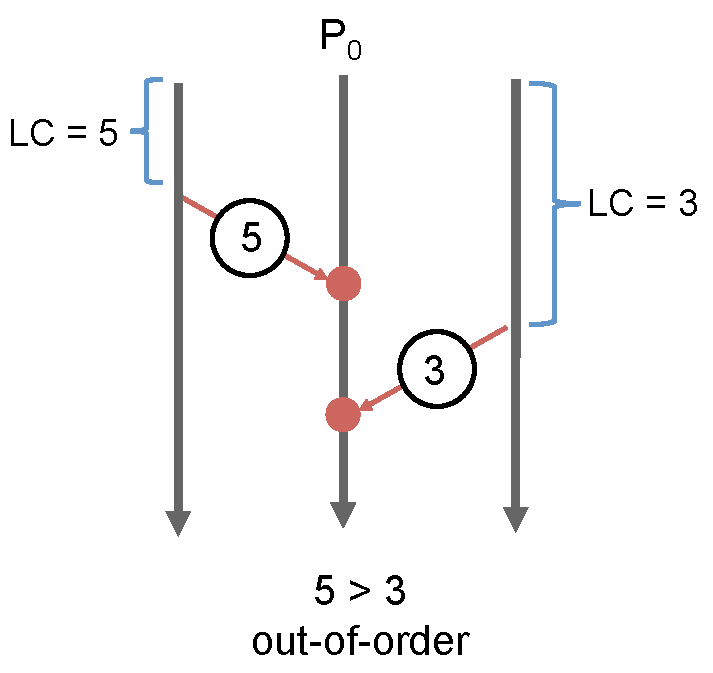
\includegraphics[width=\linewidth]{chapter_3_figures/ticking_mpisend.pdf}}
        \\ (a) Basic ticking
    \end{minipage}%
    \begin{minipage}{0.33\textwidth}
        \stackunder[5pt]{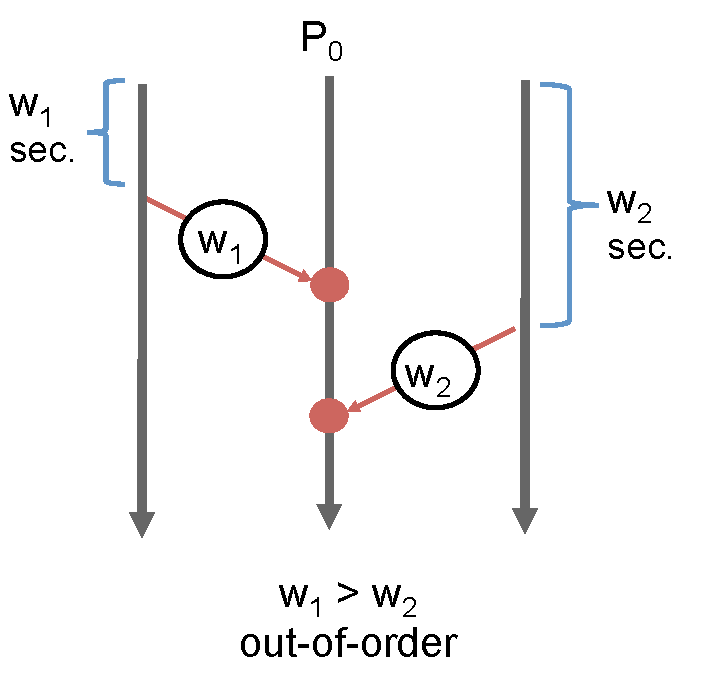
\includegraphics[width=\linewidth]{chapter_3_figures/ticking_mpiwtime.pdf}}
    \\ (b) Wall-clock ticking
    \end{minipage}%
    \begin{minipage}{0.33\textwidth}
        \stackunder[5pt]{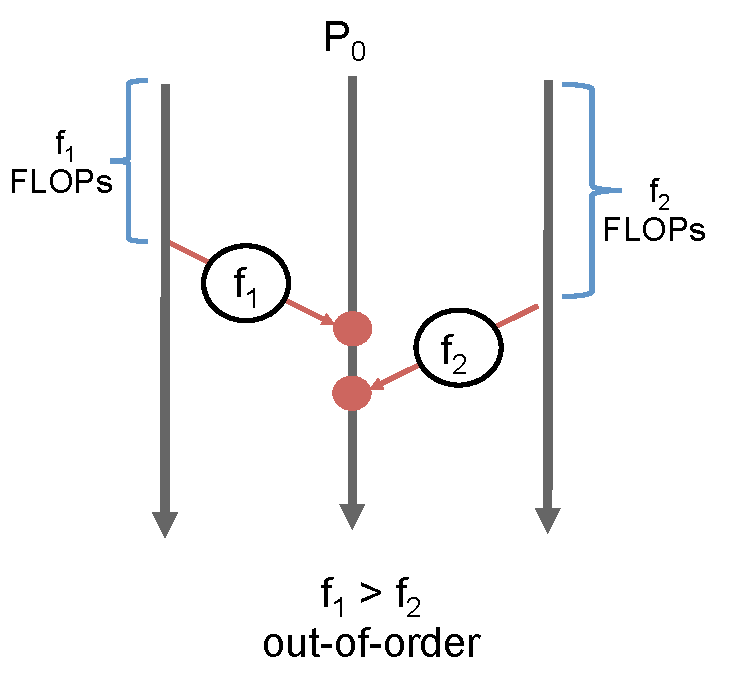
\includegraphics[width=\linewidth]{chapter_3_figures/ticking_flops.pdf}}
        \\ (c) FLOPs-based ticking
    \end{minipage}%
    \label{fig:ticking_policies}
    \caption{High level overview of the three ticking policies
      considered in this work: (a) basic ticking, (b) wall-clock
      ticking, and (c) FLOPs-based ticking.}
\end{figure}

In the message-passing HPC applications that record-and-replay tools
target, processes often alternate between progressing through
intensive floating-point workloads and communicating with other
processes. As such, we propose a FLOPs-based ticking that uses the
number of floating-point instructions completed by a process as a
proxy for wall-time. We use the Performance Application Programming
Interface (PAPI) to monitor floating-point instructions completed, and
derive ticks from those values.  Empirical investigation not shown in
this thesis indicates that the PAPI\_FP\_INS performance counter,
which measures floating-point instructions completed, yields
deterministic values, and hence deterministic ticks, when limited to
counting floating-point instructions at the application level
exclusively.  We use the MPI profiling interface (PMPI) to intercept
MPI function calls made by applications and halt PAPI's counters until
control returns to the application, as shown in
Figure~\ref{fig:ticking_policies}.(c).
 
\section{Applicability to Real Applications with Real Record-and-Replay Tool}

To evaluate the effectiveness of our PAPI\_FP\_INS-based ticking
policy in reducing the rate of out-of-order message receives, we
record multiple executions of a representative message-passing
application, the Monte Carlo Benchmark (MCB)~\cite{Software:MCB}, with a
record-and-replay tool that implements CDC, called Reproducible MPI
(ReMPI)~\cite{ClockDeltaCompression:Sato:2015}. 
In this section, we provide our rationale for
evaluating our ticking policy using MCB and ReMPI.

MCB is an MPI application that simulates particle dynamics in a domain
that is decomposed over a set of MPI processes. Particles that exit
one process's subdomain are buffered and subsequently sent to a
neighbor process's subdomain via non-blocking point-to-point
communication. MCB progresses its simulation by alternating between
three distinct communication patterns, as shown in
Figure~\ref{fig:mcb_comm_patterns}. The three patterns are:
neighbor-to-neighbor particle exchange where processes communicate
with their neighbors in a Cartesian grid; non-blocking gather where
processes are organized into a binary tree topology and send messages
to their parents in the tree; and non-blocking scatter where processes
are once again organized as a binary tree, but the direction of
communication is from parent to child.
\begin{figure}
    \centering
    \begin{minipage}{0.33\textwidth}
        \centering
        \includegraphics[width=0.9\linewidth]{chapter_3_figures/pattern_n2n}
        \\ (a) \\
    \end{minipage}% 
    \begin{minipage}{0.33\textwidth}
        \centering
        \includegraphics[width=0.9\linewidth]{chapter_3_figures/pattern_nbgather}
        \\ (b) \\
    \end{minipage}%
    \begin{minipage}{0.33\textwidth}
        \centering
        \includegraphics[width=0.9\linewidth]{chapter_3_figures/pattern_nbscatter}
         \\ (c) \\
    \end{minipage}%
    \caption{MCB communication patterns: the neighbor-to-neighbor
      particle exchange (a), the non-blocking gather (b), and the
      non-blocking scatter (c).}
    \label{fig:mcb_comm_patterns}
\end{figure}
MCB is known to exhibit non-deterministic communication due to its use
of non-blocking point-to-point communication and wildcard receives
(i.e., allowing a pending receive request to match with the first
message that arrives), rather than a message from a specific
sender. Moreover, run-to-run variability in MCB's numerical outputs
has been observed~\cite{Reproducibility:Cleveland:2013} that is
attributable to non-deterministic communication. Consequently, MCB is
an ideal candidate application for testing a record-and-replay tool.

We implement our ticking policies in ReMPI. ReMPI is, to the best
of our knowledge, the only record-and-replay tool that implements
CDC. Additionally, ReMPI's design as a composition of PMPI
modules~\cite{PMPI:Dongarra:1995}~\cite{PNMPI:Schulz:2007} simplified
the implementation of our ticking policy. By default ReMPI uses
the basic ticking policy where all ticks are set to $1$.

\section{Assessing Different Ticking Policies}

We compare our ticking policy based on floating-point operations
against the baseline ReMPI ticking policy. In our analysis we consider
the effect of application-level parameters (i.e., floating-point
workload per process and rate of messaging between processes) on the
rate of out-of-order messages.

\subsection{Experimental Setting}

By varying the number of particles that each MPI process initially
simulates, we can effectively vary the intensity of each process's
floating-point workload (i.e., the more particles are simulated per
process, the more floating point operation are performed). Note that
we consider a homogeneous distributed of particles per process. By
varying the size of the communication buffer between two processes
each process uses to accumulate particles en-route to a neighbor
process, we can effectively vary the rate of communication (i.e., by
decreasing the buffer size we increase the number of messages
issued). In Figure~\ref{fig:parameter_matrix} we show the four
scenarios we test in this thesis (in green). We consider either 1K or
1M particles for process and either a buffer size containing data for
5 or for 5,000 particles leaving a process subdomain for the neighbor
process sharing the buffer.
\begin{figure}[!ht]
    \centering
    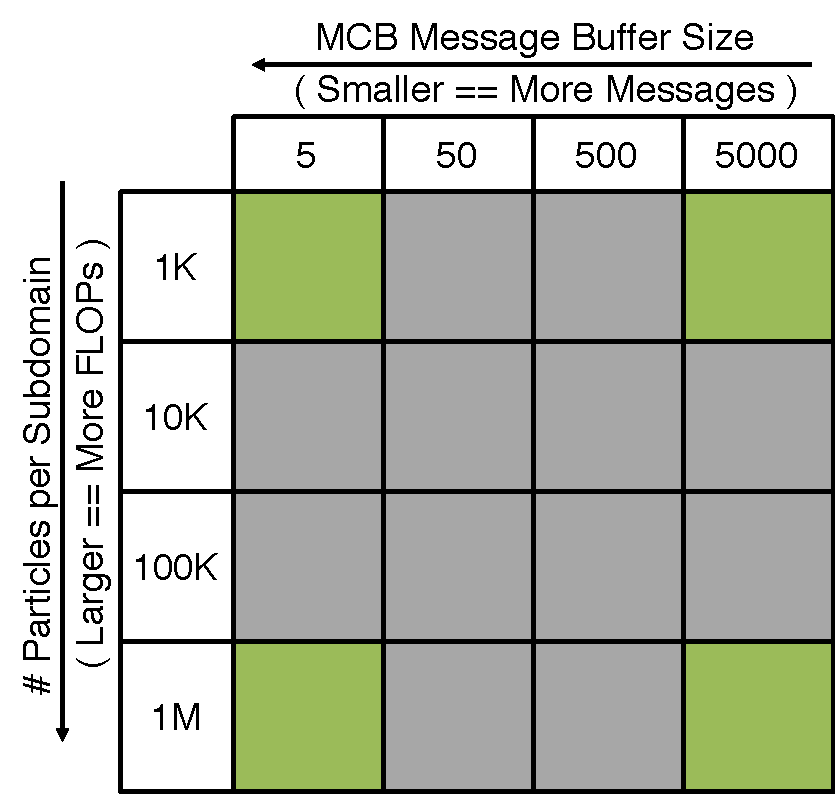
\includegraphics[width=0.5\linewidth]{chapter_3_figures/parameter_matrix.pdf}
    \caption{Tested scenarios (in green cells) in the space of
      application parameters considered in this thesis. Gray cells are
      left for future work.}
    \label{fig:parameter_matrix}
\end{figure}

For each one of the four MCB scenarios we evaluate our FLOPs-based
ticking (referred in the figures in the next section as
PAPI\_FP\_INS-ticking) against the baseline ticking policy built into
ReMPI (hereafter referred to as MPI\_SEND-ticking) and a
non-replayable wall-time-based ticking policy (referred to as
MPI\_WTIME-ticking). For each scenario and each ticking policy, we
record $100$ executions of MCB with the extended ReMPI set to log the
number of messages received in-order and the number of messages
received out-of-order by each MPI process. For each process, we
compute the percentage of messages received out-of-order, and then
aggregate these percentages across all $100$ executions, thereby
obtaining a global view of the ticking policies' effectiveness at
minimizing the rate of out-of-order messages.

We conduct our tests on Vulcan, a BlueGene/Q cluster at Lawrence
Livermore National Laboratory. Each node of Vulcan consists of 16 1.6
GHz PowerA2 processors and is equipped with 16 GB of RAM.  The nodes
are networked to each other in a 5D torus. We consider three scenarios
consisting of one single node running a 16-processes MCB, four nodes
running a 64-processes MCB, and 16 nodes running a 256-processes MCB.

\subsection{Results} \label{subsec:results}

Figures~\ref{fig:resutls1} plot the distributions of out-of-order
message percentages for each ticking policy and the median
out-of-order percentage for each ticking policy over all executions on
a single node of Vulcan.
\begin{figure}[!htb]
    \begin{minipage}[b]{0.5\linewidth}
        \centering
        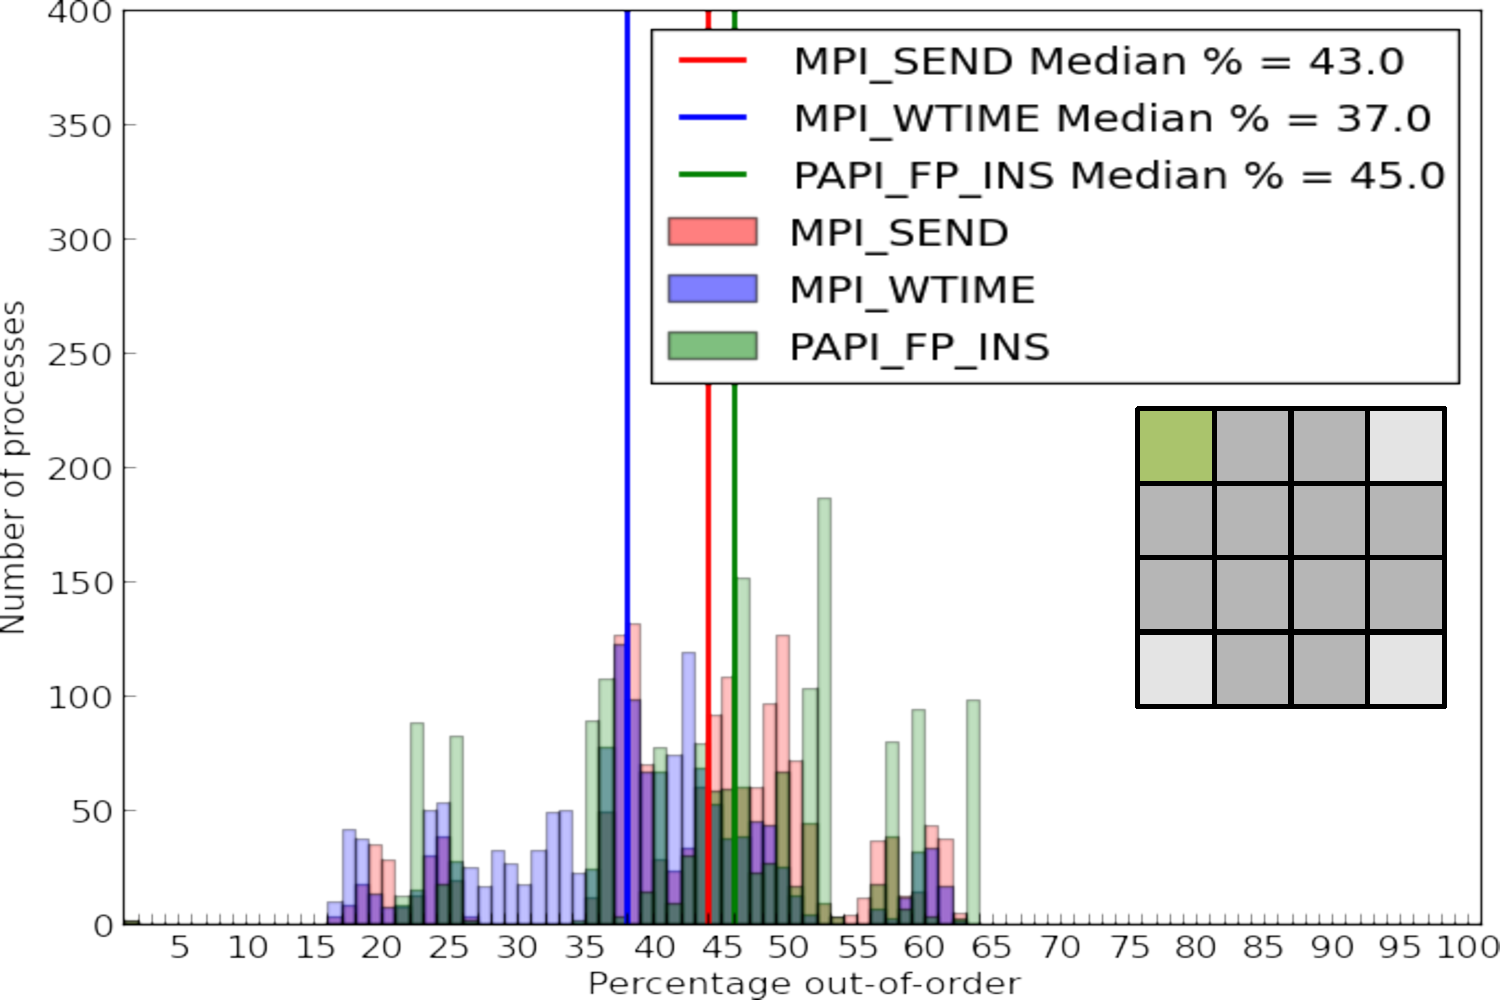
\includegraphics[width=0.95\linewidth]{chapter_3_figures/hist_nodes1_procs16_particles1000_cycles10_bufferSize5.pdf} 
        \\ (a) \\
    \end{minipage}
    \begin{minipage}[b]{0.5\linewidth}
        \centering
        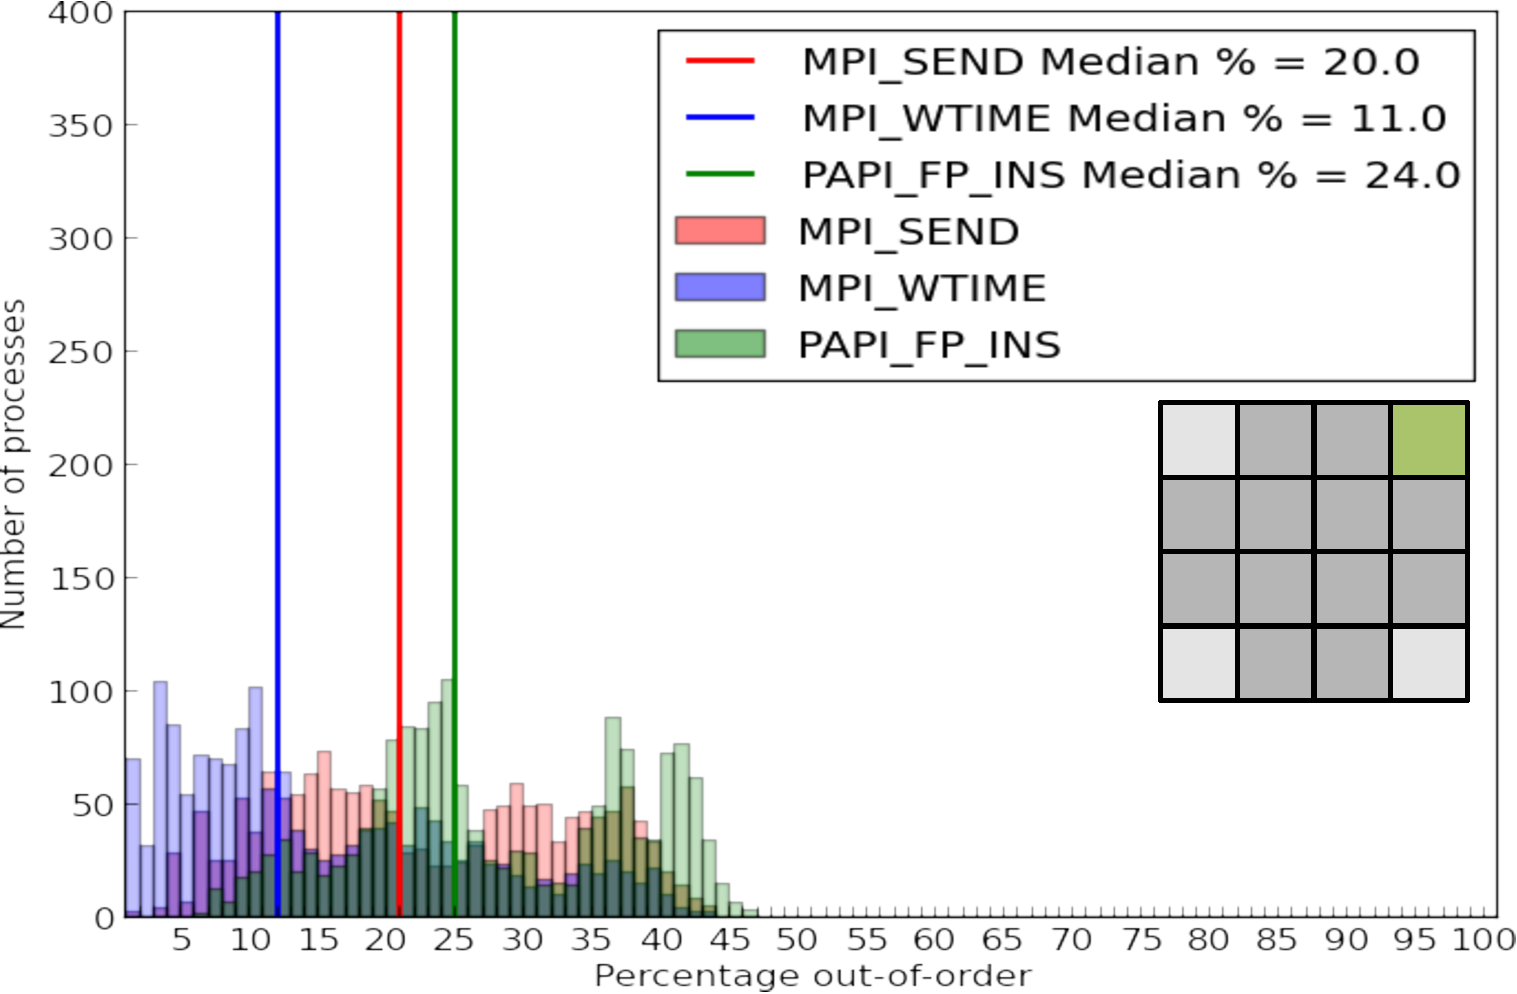
\includegraphics[width=0.95\linewidth]{chapter_3_figures/hist_nodes1_procs16_particles1000_cycles10_bufferSize5000.pdf}
        \\ (b) \\
    \end{minipage}
    \begin{minipage}[b]{0.5\linewidth}
        \centering
        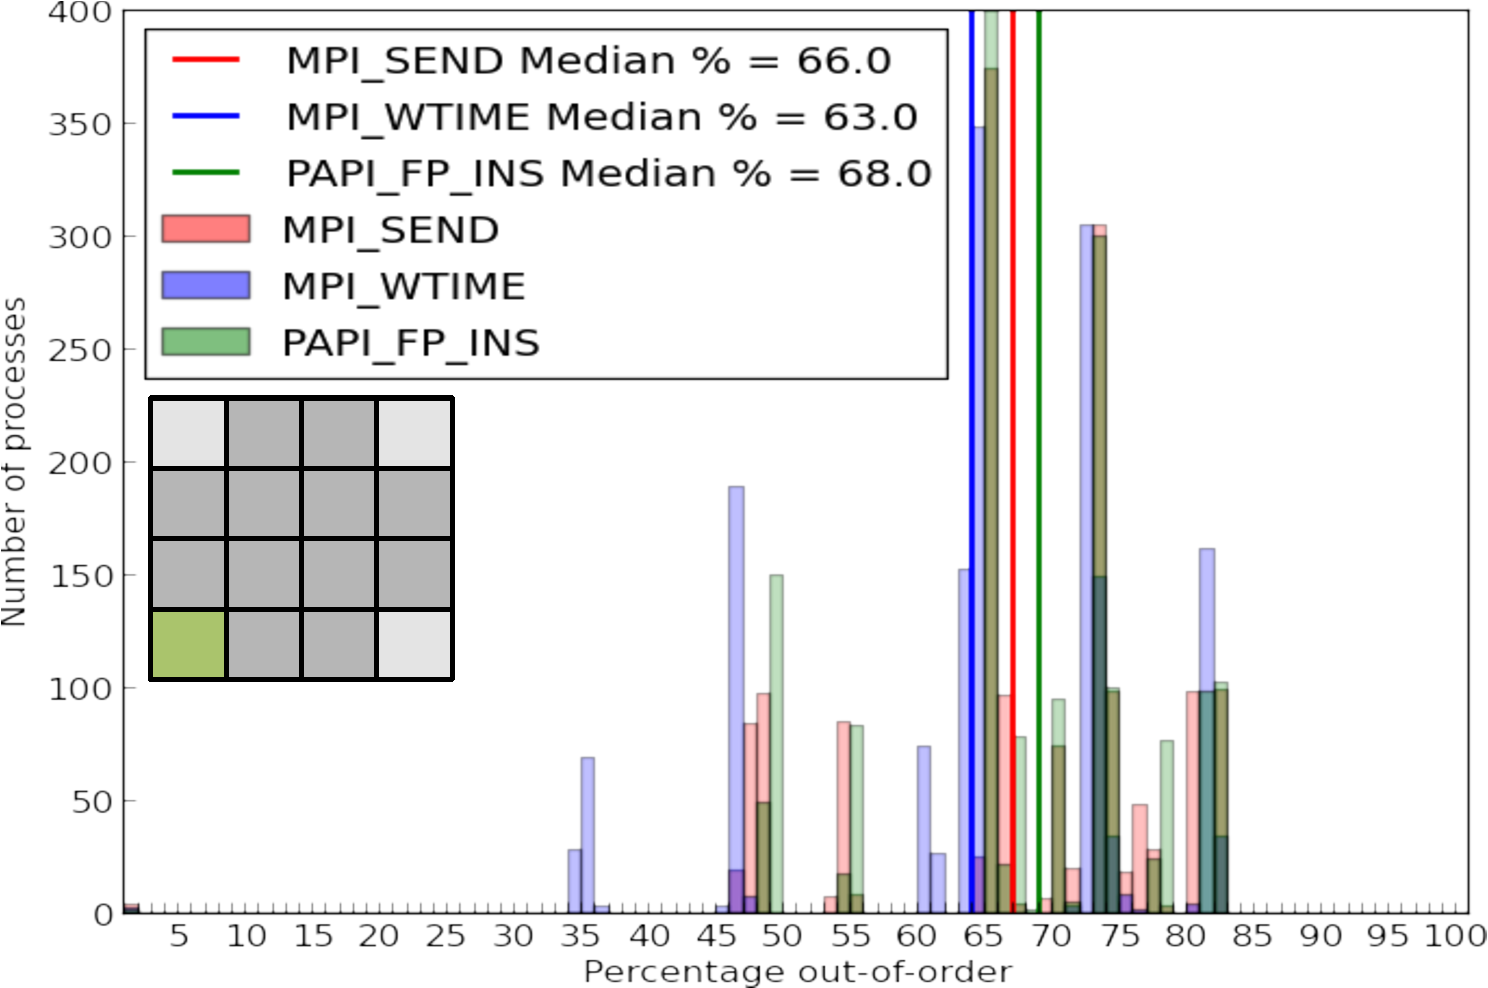
\includegraphics[width=0.95\linewidth]{chapter_3_figures/hist_nodes1_procs16_particles1000000_cycles10_bufferSize5.pdf}
        \\ (c) \\
    \end{minipage}
    \begin{minipage}[b]{0.5\linewidth}
        \centering
        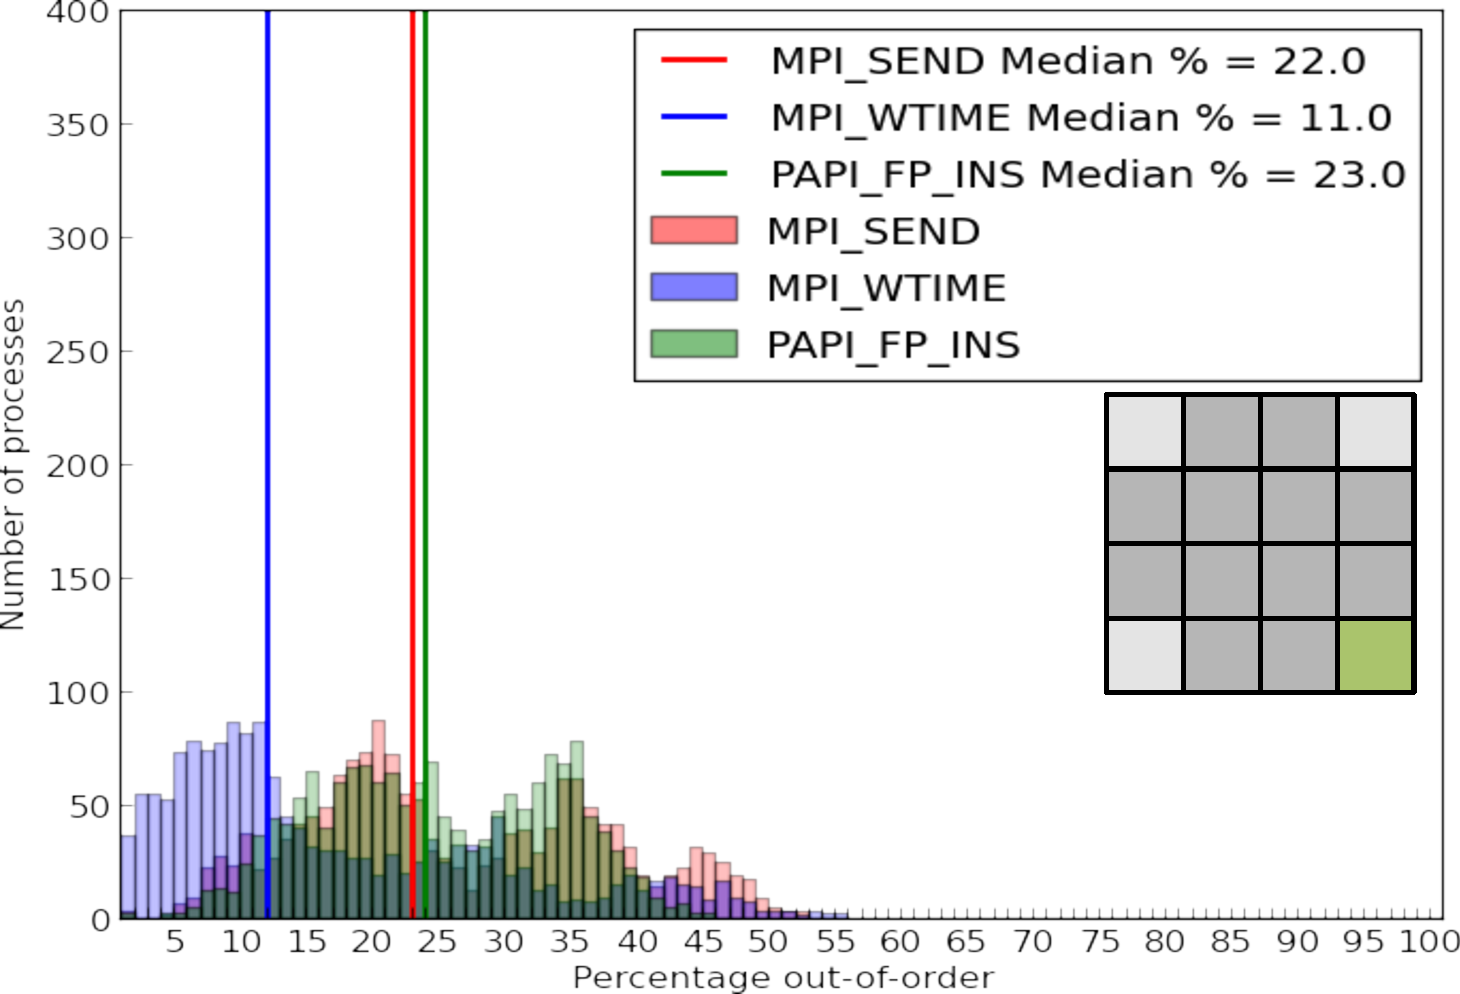
\includegraphics[width=0.95\linewidth]{chapter_3_figures/hist_nodes1_procs16_particles1000000_cycles10_bufferSize5000.pdf}
       \\ (d) \\
    \end{minipage}
    \caption{Distributions of out-of-order message percentages and
      median out-of-order percentage for each ticking policy over all
      executions on a \textbf{single node} of Vulcan. 
      The test cases are: 
      1K particles per process, buffer size 5 (a); 
      1K particles per process, buffer size 5K (b);
      1M particles per process, buffer size 5 (c);
      and 1M particles per process, buffer size 5K (d).}
    \label{fig:resutls1}
\end{figure}
At the single-node scale, we observe that MPI\_WTIME-ticking improves
the median out-of-order message percentage relative to
MPI\_SEND-ticking best when communication intensity is low (i.e., when
the MCB buffer size is large). The median improvement is $9\%$ in the
low floating-point workload case, and $11\%$ in the high
floating-point workload case. Conversely, when the communication
intensity is high due to a small MCB buffer size, the improvement
MPI\_WTIME-ticking offers is minimized--$6\%$ and $3\%$
respectively. We conjecture that this is due to the fact that when
more messages are sent per unit of wall-clock time, ticking by $1$ per
message send more closely resembles the passage of wall-clock time
than in the case where message sends are less frequent. In all four
cases however, we note that the PAPI\_FP\_INS-based ticking does not
improve the median out-of-order percentage relative to
MPI\_SEND-ticking, contrary to our expectation. We do note however
that in the low communication intensity and high floating-point
workload case, the out-of-order message rate of PAPI\_FP\_INS-ticking
closely approaches that of MPI\_SEND-ticking.

In the four-node tests shown in Figures~\ref{fig:resutls4}, we
observe that while MPI\_WTIME-ticking continues to excel in the low
communication intensity cases, MPI\_SEND-ticking matches it very
closely in the high communication intensity cases, even slightly
exceeding it when the per-process floating-point workload is also
low. Also notable is that in the two high floating-point workload
cases, PAPI\_FP\_INS-ticking matches very closely with
MPI\_SEND-ticking, lending further credence to the idea that
PAPI\_FP\_INS-ticking can be useful for applications where per-process
floating-point workload strongly influences the timing of message
sends.
\begin{figure}[!htb]
    \begin{minipage}[b]{0.5\linewidth}
        \centering
        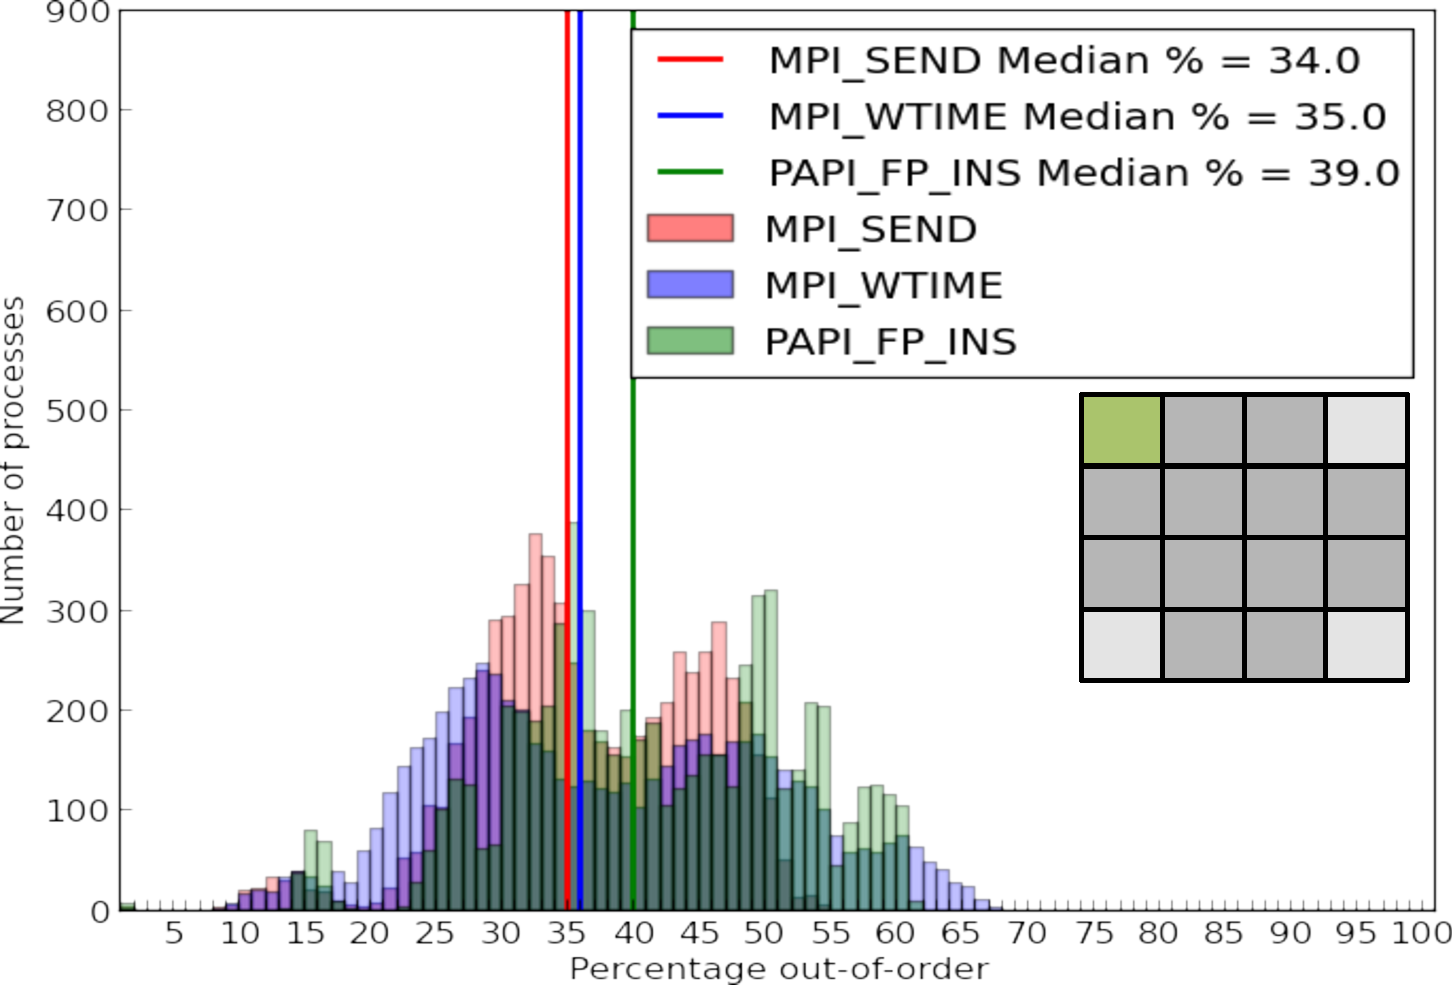
\includegraphics[width=0.95\linewidth]{chapter_3_figures/hist_nodes4_procs64_particles1000_cycles10_bufferSize5.pdf}
        \\ (a) \\
    \end{minipage}
    \begin{minipage}[b]{0.5\linewidth}
        \centering
        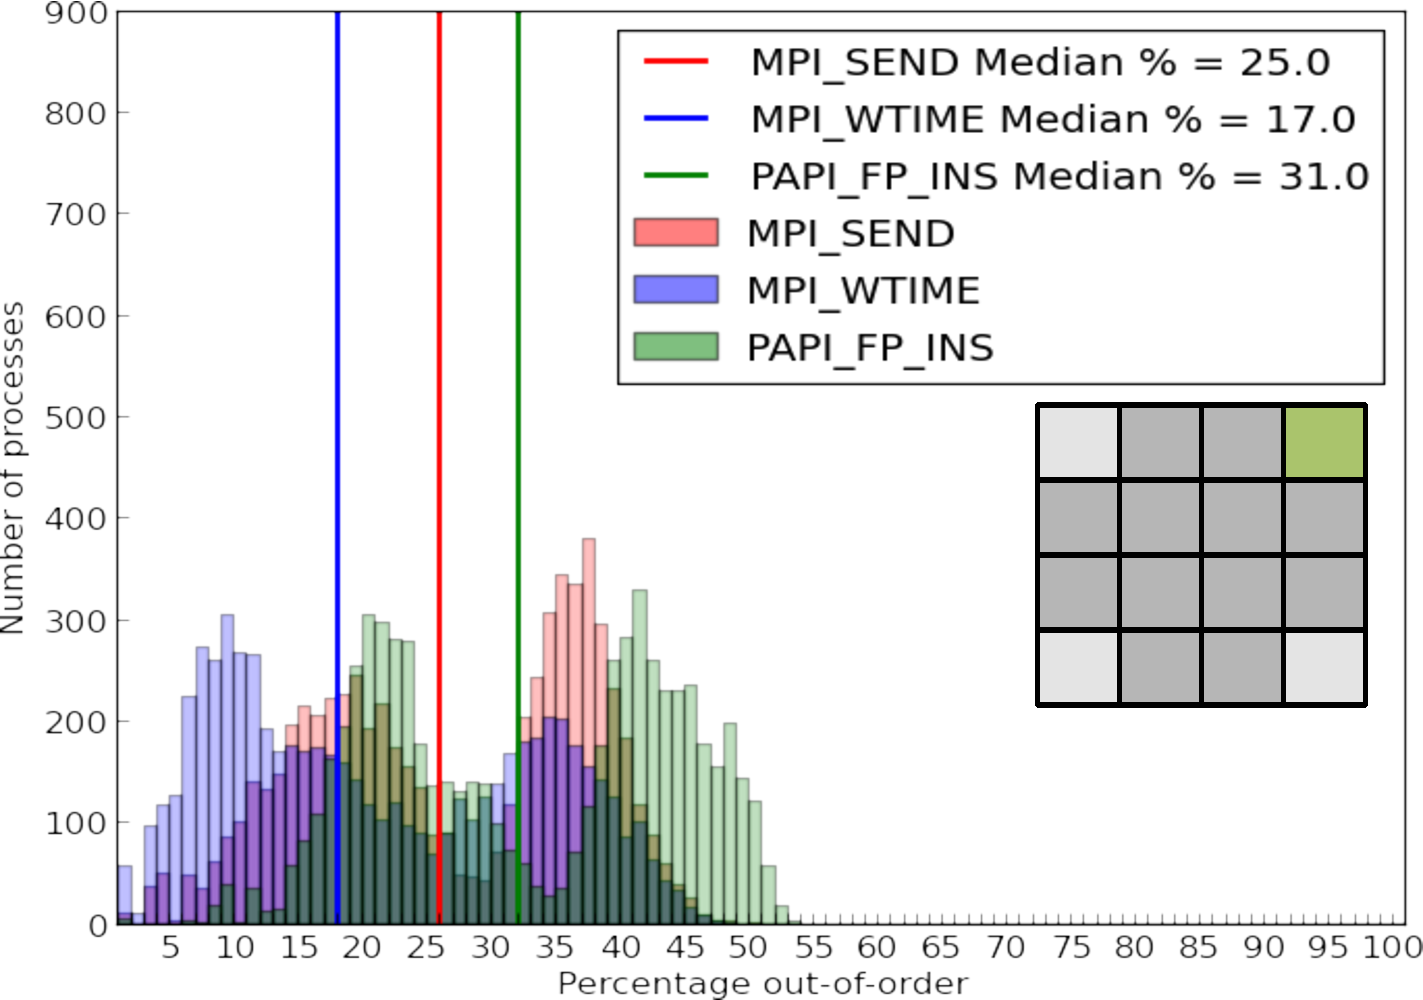
\includegraphics[width=0.95\linewidth]{chapter_3_figures/hist_nodes4_procs64_particles1000_cycles10_bufferSize5000.pdf}
        \\ (b) \\
    \end{minipage}
    \begin{minipage}[b]{0.5\linewidth}
        \centering
        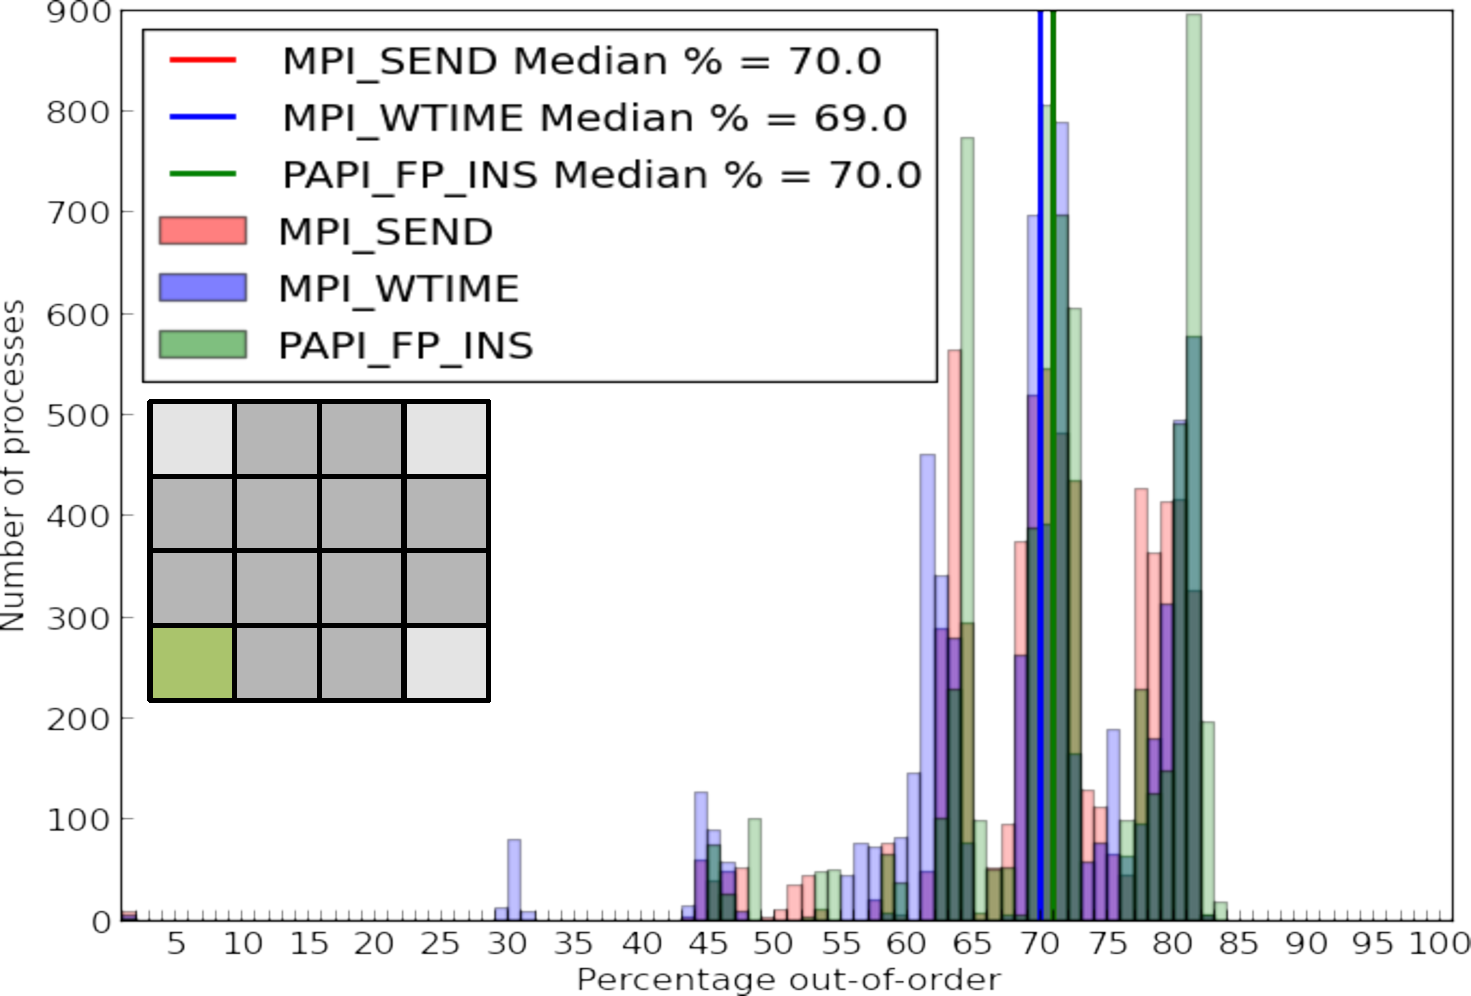
\includegraphics[width=0.95\linewidth]{chapter_3_figures/hist_nodes4_procs64_particles1000000_cycles10_bufferSize5.pdf}
        \\ (c) \\
    \end{minipage}
    \begin{minipage}[b]{0.5\linewidth}
        \centering
        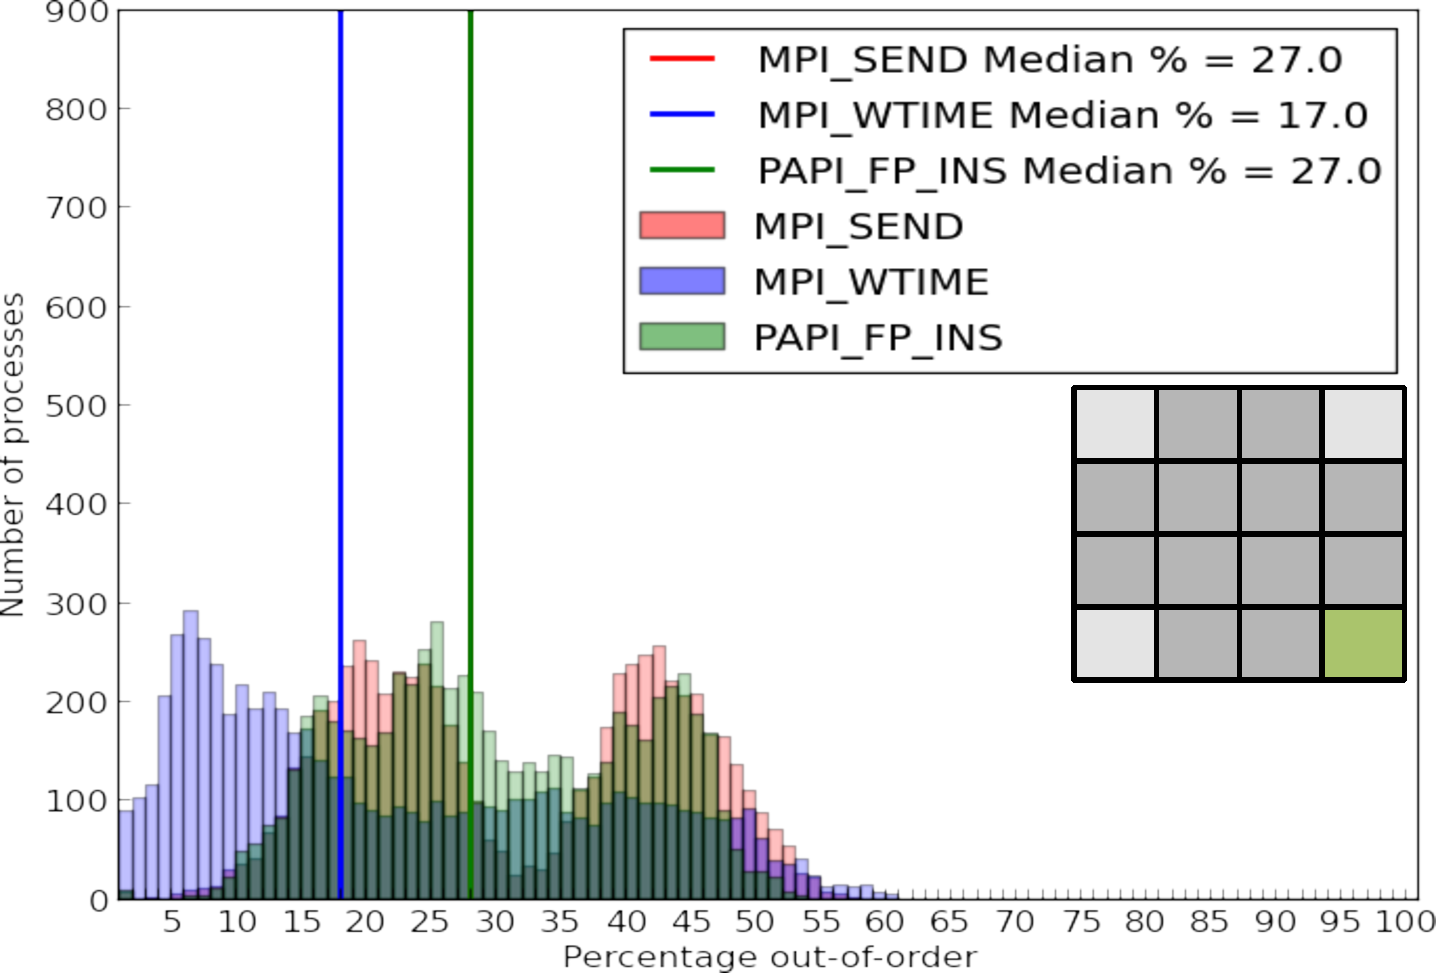
\includegraphics[width=0.95\linewidth]{chapter_3_figures/hist_nodes4_procs64_particles1000000_cycles10_bufferSize5000.pdf}
       \\ (d) \\
    \end{minipage}
    \caption{Distributions of out-of-order message percentages and
      median out-of-order percentage for each ticking policy over all
      executions on \textbf{four nodes} of Vulcan.
      The test cases are: 
      1K particles per process, buffer size 5 (a); 
      1K particles per process, buffer size 5K (b);
      1M particles per process, buffer size 5 (c);
      and 1M particles per process, buffer size 5K (d).}
    \label{fig:resutls4}  
\end{figure}

At the 16-node scale shown in Figures~\ref{fig:resutls16}, we observe
that even in the low communication intensity, low floating-point
workload case, MPI\_SEND-ticking gets very close to the performance of
MPI\_WTIME-ticking. The trend we have so far observed of strong
agreement between all three ticking policies in the high communication
intensity, high floating-point workload case continues, as does the
trend of strong agreement between MPI\_SEND-ticking and
PAPI\_FP\_INS-ticking in the low communication intensity, high
floating-point workload case.
\begin{figure}[!htb]
    \begin{minipage}[b]{0.5\linewidth}
        \centering
        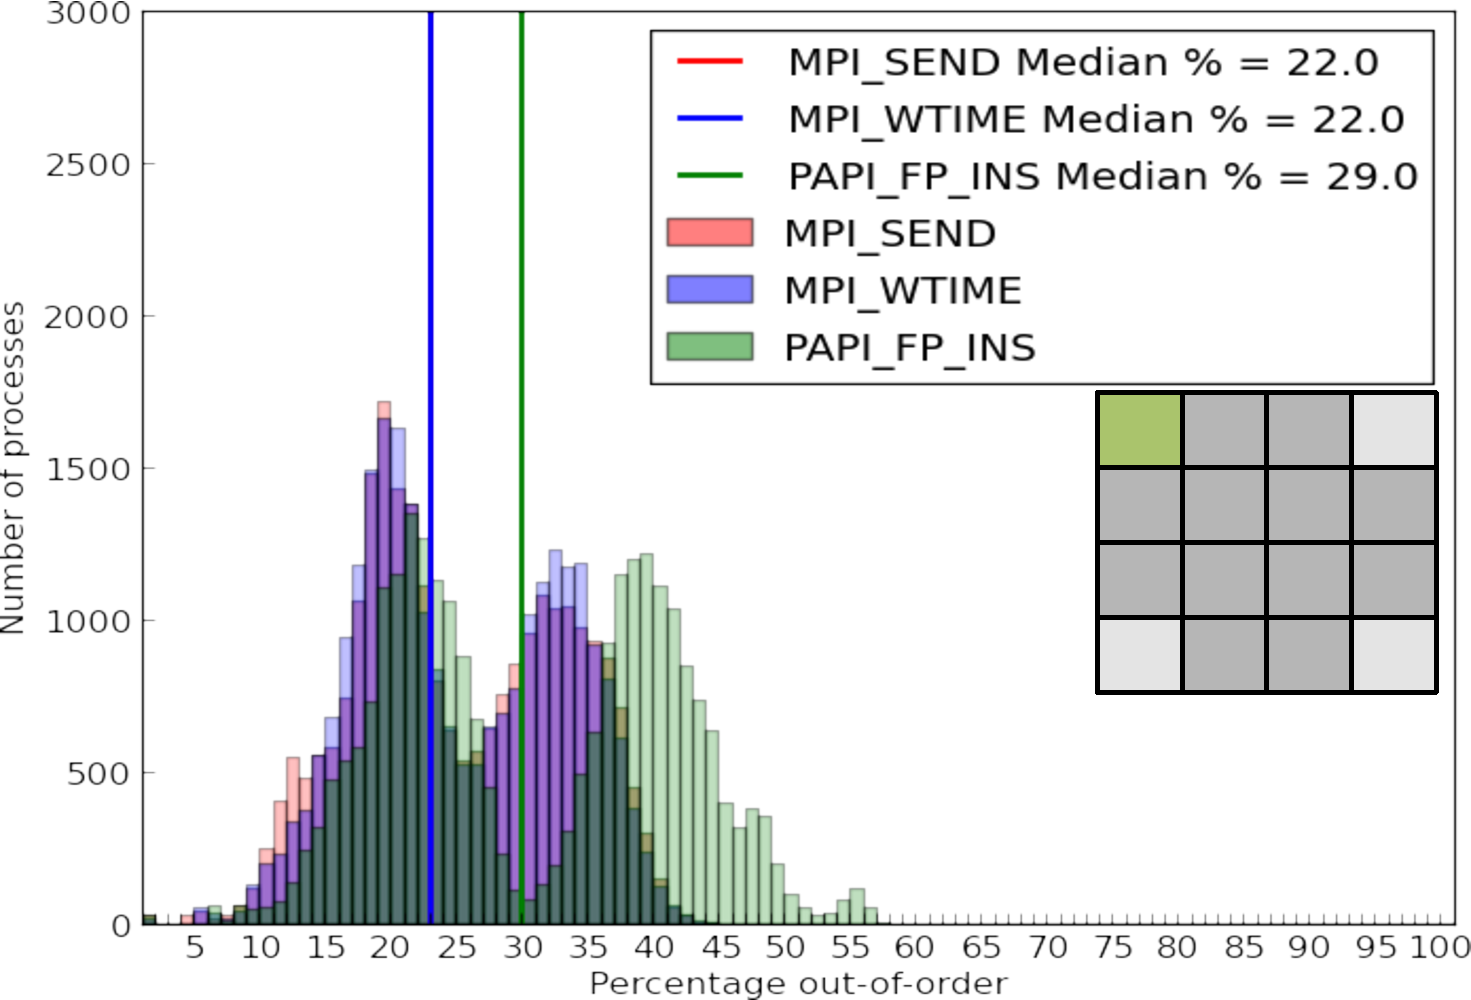
\includegraphics[width=0.95\linewidth]{chapter_3_figures/hist_nodes16_procs256_particles1000_cycles10_bufferSize5.pdf}
        \\ (a) \\
    \end{minipage}
    \begin{minipage}[b]{0.5\linewidth}
        \centering
        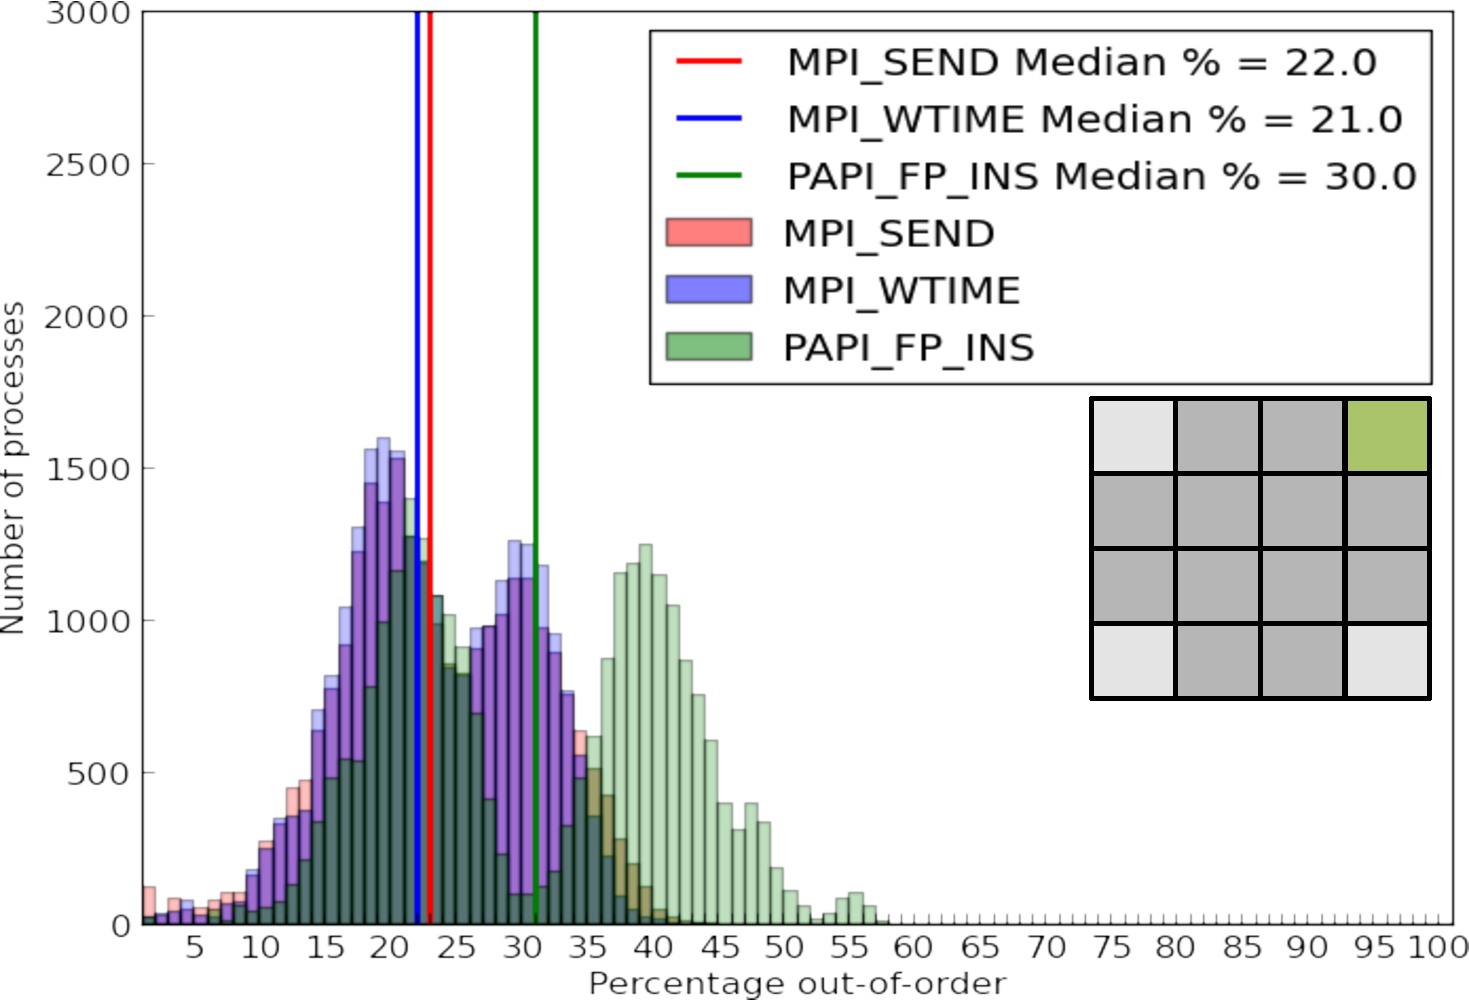
\includegraphics[width=0.95\linewidth]{chapter_3_figures/hist_nodes16_procs256_particles1000_cycles10_bufferSize5000.pdf}
        \\ (b) \\
    \end{minipage}
    \begin{minipage}[b]{0.5\linewidth}
        \centering
        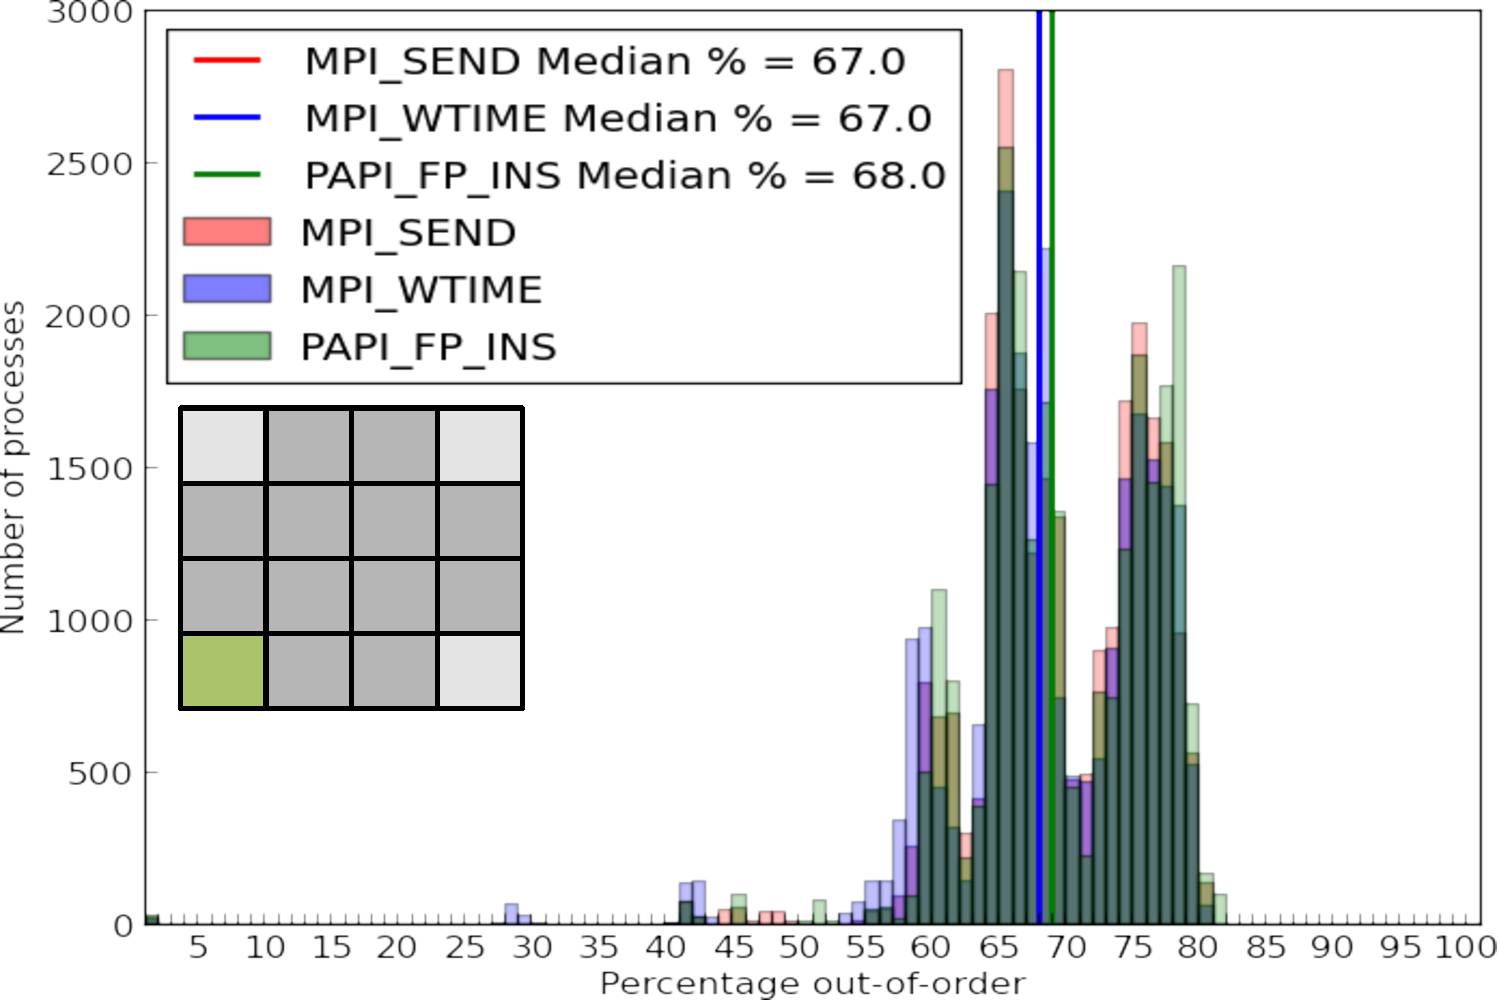
\includegraphics[width=0.95\linewidth]{chapter_3_figures/hist_nodes16_procs256_particles1000000_cycles10_bufferSize5.pdf}
       \\ (c) \\
    \end{minipage}
    \begin{minipage}[b]{0.5\linewidth}
        \centering
        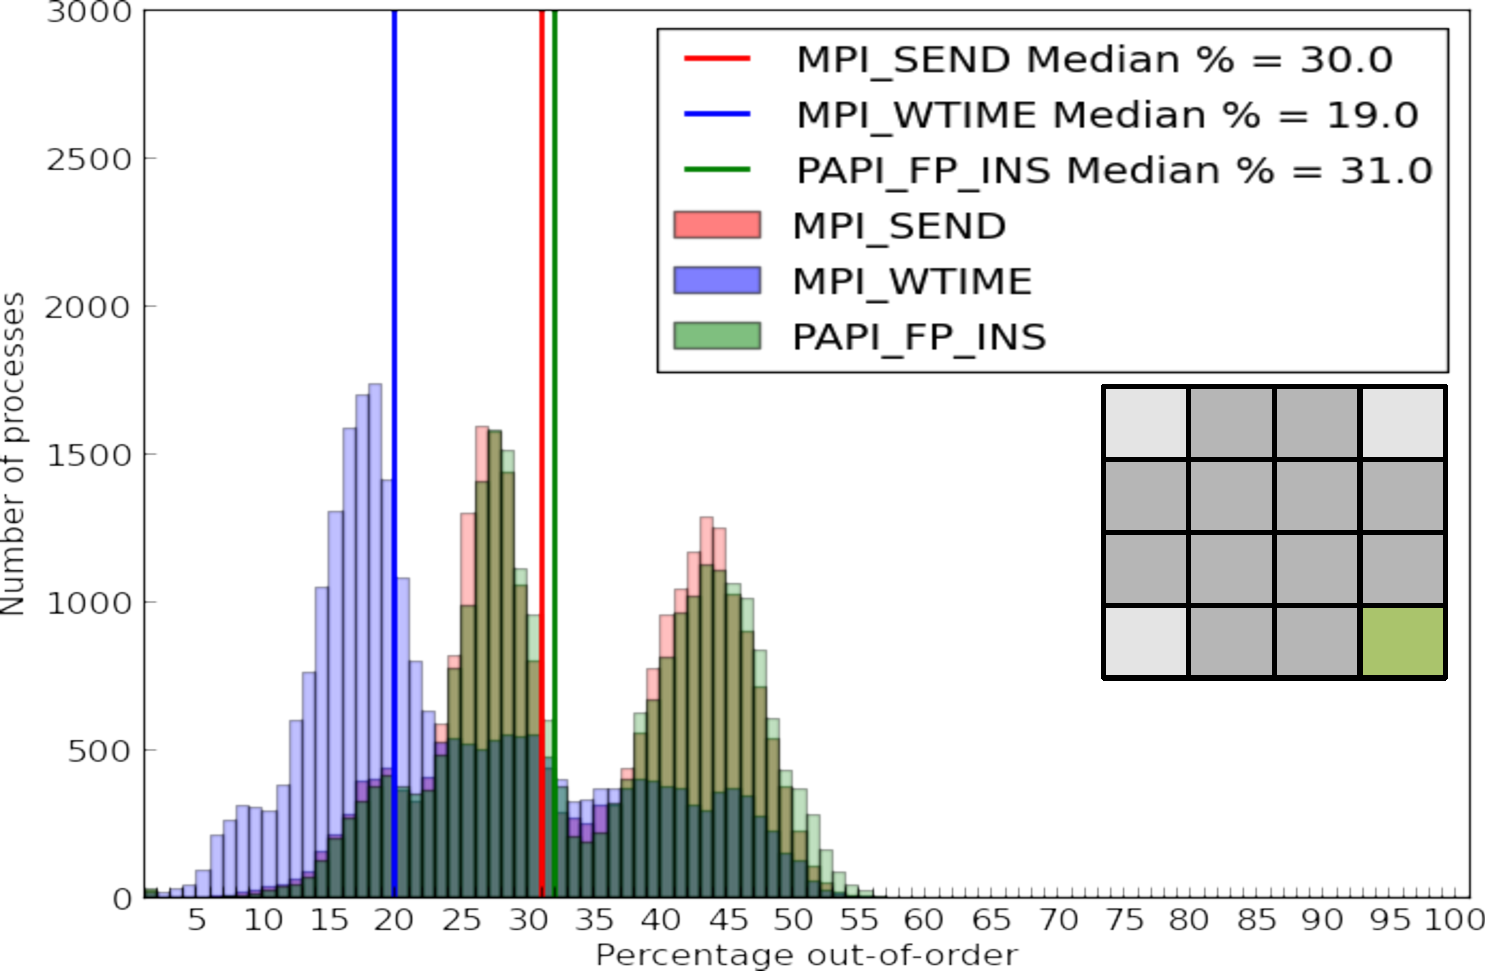
\includegraphics[width=0.95\linewidth]{chapter_3_figures/hist_nodes16_procs256_particles1000000_cycles10_bufferSize5000.pdf}
        \\ (d) \\
    \end{minipage}
    \caption{Distributions of out-of-order message percentages and
      median out-of-order percentage for each ticking policy over all
      executions on \textbf{16 nodes} of Vulcan.
      The test cases are: 
      1K particles per process, buffer size 5 (a); 
      1K particles per process, buffer size 5K (b);
      1M particles per process, buffer size 5 (c);
      and 1M particles per process, buffer size 5K (d).}
    \label{fig:resutls16}  
\end{figure}

\section{Lessons Learned}

The work in this chapter was motivated from the question whether a
ticking policies that resembles the non-replayable wall-clock ticking
policy such as our FLOPs-based ticking policies can outperform the
baseline ticking policy built into ReMPI. 

By comparing the performances of our 
FLOPs-based ticking against the baseline ticking policy built into
ReMPI and a non-replayable wall-time-based ticking policy in four
distinct scenarios, we have begun to develop insight into the
interaction between application behaviors and the effectiveness of
different ticking policies. Although we were not able to observe
improvement in median out-of-order percentage for the baseline
ticking policy built into our FLOPs-based ticking relative to the
baseline ticking policy built into ReMPI, we posit that our ticking
policy may still form the basis of a future ticking policy that takes
additional application-level information into account to reduce the
out-of-order message rate. Additionally, we posit that applications
exhibiting greater imbalance between processes' floating-point
workloads may benefit more from FLOPs-based ticking policies than MCB
does. 

One aspect we need to consider is that the MCB application does not
have one single communication pattern that is a source of
non-determinism, In other words, the tests we showed in this chapter
do not identify whether the out-of-order messages are more caused by one
of the three patterns. This aspect is further discussed in the next
chapter.
